\subsection*{Problema 18}

\textbf{Enunciado:} Calcular la integral:
\begin{align*}
\int \dfrac{x^2 - 1}{(x^2 + 1)(x - 2)} \, dx
\end{align*}

\textbf{Solución:} \\
Utilizamos el método de fracciones parciales. 
Planteamos la descomposición indicada:
\begin{align*}
\dfrac{x^2 - 1}{(x^2 + 1)(x - 2)} &= \dfrac{Ax + B}{x^2 + 1} + \dfrac{C}{x - 2}
\end{align*}

Multiplicando ambos lados por el denominador común:
\begin{multline*}
x^2 - 1 = (Ax + B)(x - 2) \\
+ C(x^2 + 1)
\end{multline*}

Expandimos el miembro derecho:
\begin{multline*}
x^2 - 1 = Ax^2 - 2Ax + Bx \\
- 2B + Cx^2 + C
\end{multline*}

Agrupamos términos según las potencias de $x$:
\begin{multline*}
x^2 - 1 = (A + C)x^2 \\
+ (-2A + B)x + (-2B + C)
\end{multline*}

Igualamos los coeficientes:
\begin{align*}
A + C &= 1 \\
-2A + B &= 0 \\
-2B + C &= -1
\end{align*}

De la segunda ecuación, $B = 2A$. 
Sustituyendo $C = 1 - A$ y $B = 2A$ en la tercera:
\begin{align*}
-2(2A) + (1 - A) &= -1 \\
-4A + 1 - A &= -1 \\
-5A &= -2 \implies A = \dfrac{2}{5}
\end{align*}

Calculamos $B$ y $C$:
\begin{align*}
B &= 2\left(\dfrac{2}{5}\right) = \dfrac{4}{5} \\
C &= 1 - \dfrac{2}{5} = \dfrac{3}{5}
\end{align*}

Sustituimos los coeficientes:
\begin{multline*}
\int \dfrac{x^2 - 1}{(x^2 + 1)(x - 2)} \, dx = 
\int \dfrac{\frac{2}{5}x + \frac{4}{5}}{x^2 + 1} \, dx \\
+ \int \dfrac{\frac{3}{5}}{x - 2} \, dx
\end{multline*}

Resolvemos cada integral por separado:
\begin{align*}
&= \dfrac{1}{5} \int \dfrac{2x}{x^2 + 1} \, dx \\
&\quad + \dfrac{4}{5} \int \dfrac{1}{x^2 + 1} \, dx \\
&\quad + \dfrac{3}{5} \int \dfrac{1}{x - 2} \, dx
\end{align*}

Integrando cada término:
\begin{multline*}
= \dfrac{1}{5} \ln|x^2 + 1| \\
+ \dfrac{4}{5} \arctan(x) \\
+ \dfrac{3}{5} \ln|x - 2| + K
\end{multline*}

La solución general de la integral es:
\begin{multline*}
F(x) = \dfrac{1}{5} \ln(x^2 + 1) \\
+ \dfrac{4}{5} \arctan(x) \\
+ \dfrac{3}{5} \ln|x - 2| + C
\end{multline*}

\begin{figure}[H]
	\centering
	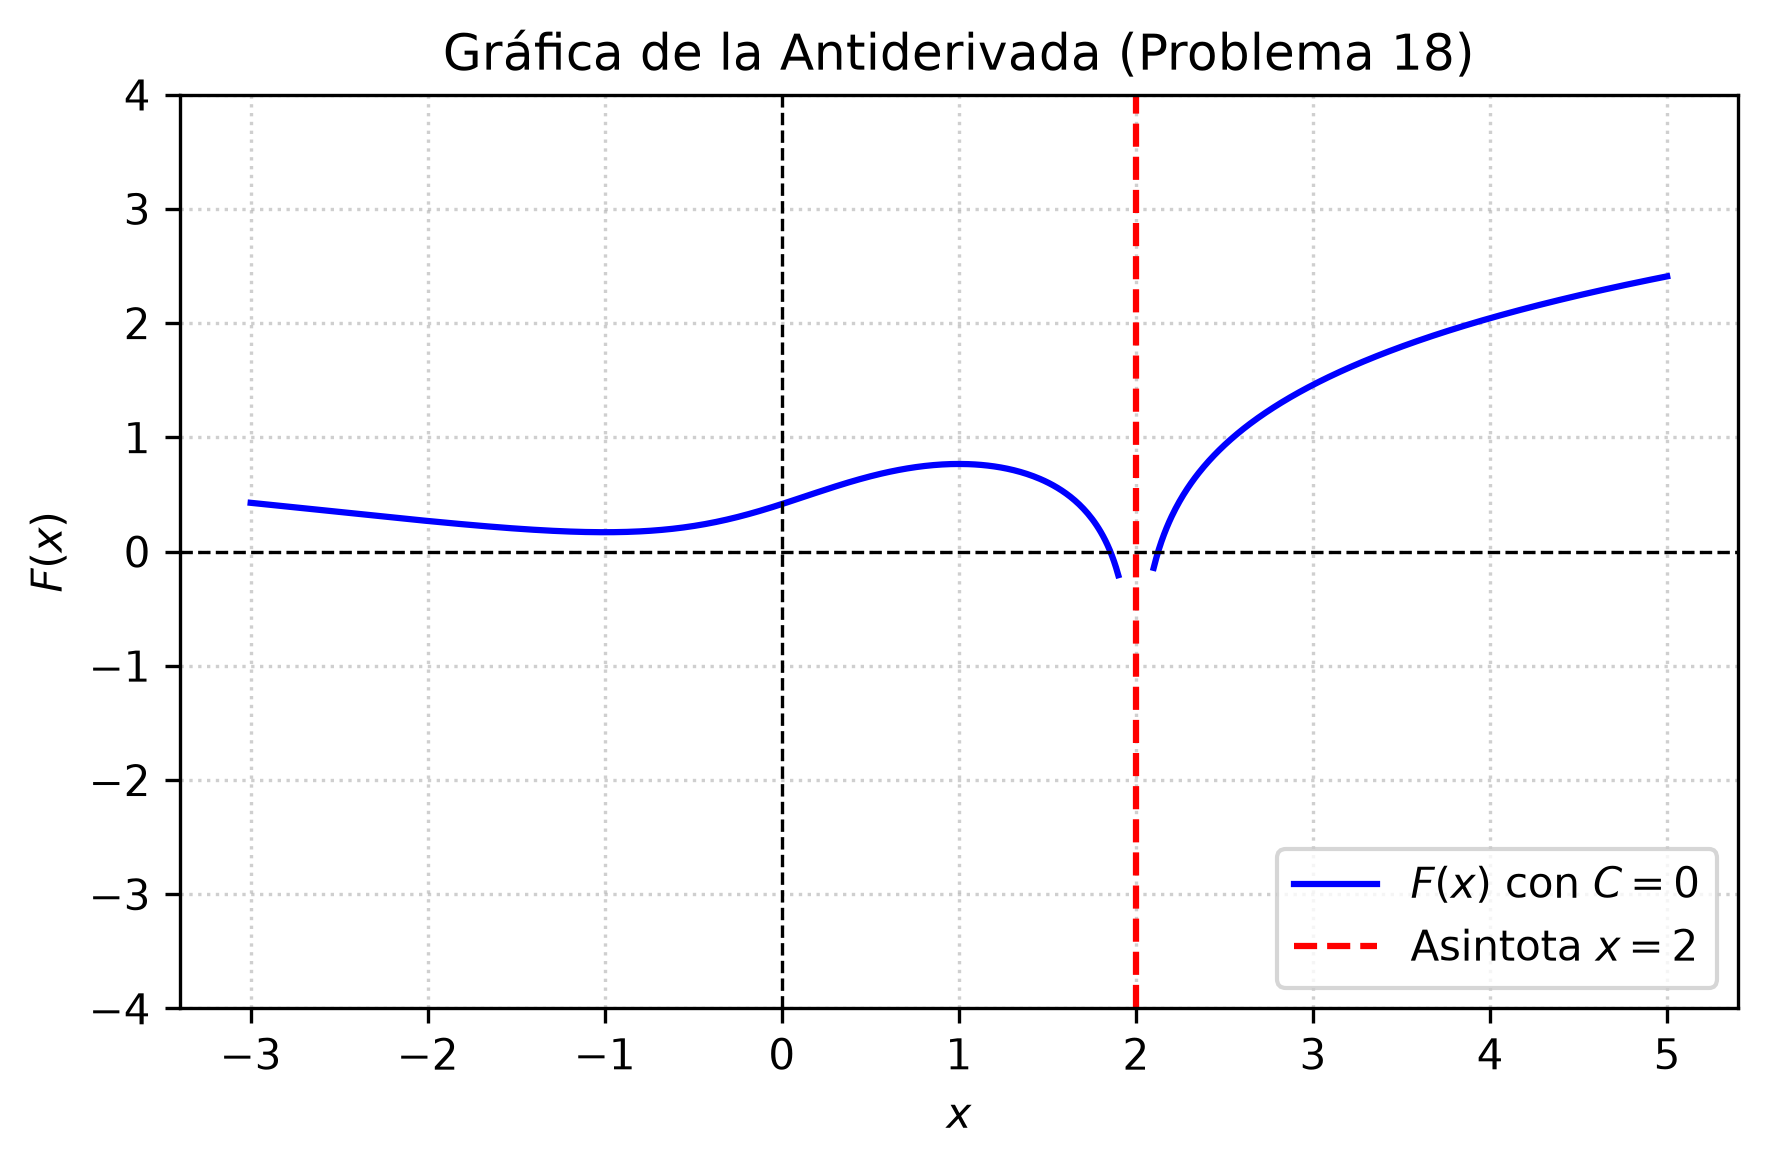
\includegraphics[width=\columnwidth]{semana_03/graficas/SEM03_P18_grafica.png}
	\caption{Representación gráfica de $f(x)$ y su antiderivada $F(x)$ evaluada para la constante de integración $C = 0$ (Problema 18).}
	\label{fig:problema18}
\end{figure}
